\section{Raporty o stanie techniki jako informacja o dyfuzji}

Na stronie \ac{UPRP} wyróżniono etapy w procesie patentowania.
Etapem po spełnieniu formalności jest 
\textit{sprawozdanie ze stanu techniki}\cite{UPRP-pat-prd}.
Słownik urzędu wskazuje, że \textit{stan techniki} to wszelka
wiedza dostępna do wskazanej daty powszechnie, albo taka,
która nie jest publiczna, ale została już ogłoszona 
w określony sposób\cite{UPRP-dict}.

Sprawozdanie jest realizowane przez urzędników i składa się z
klasyfikacji zgłoszenia, informacji o innych klasyfikacjach,
w których prowadzono poszukiwania, wykaz baz komputerowych,
użytych w trakcie procesu oraz tabelę zawierającą odniesienia
do innych prac. Wśród odniesień można wyróżnić odniesienia do
patentów, artykułów naukowych, książek, stron internetowych,
a także do innych zgłoszeń patentowych.
Przykłady takich odniesień są przedstawione na następnej stronie.

\newpage
\begin{figure}[H]\centering
\label{fig:raport-biblio-ex}
\includegraphics[width=0.8\textwidth]{ex-img/bilblio-ex-1.jpg}
\caption{Przykład odniesienia do literatury technicznej 
         w raporcie o stanie techniki.}
\end{figure}
\begin{figure}[H]\centering
\label{fig:raport-pat-ex}
\includegraphics[width=0.8\textwidth]{ex-img/pat-ex-1.jpg}
\caption{Przykład odniesienia do innych patentów 
         w raporcie o stanie techniki.}
\end{figure}
\begin{figure}[H]\centering
\label{fig:raport-url-ex}
\includegraphics[width=0.8\textwidth]{ex-img/url-ex-1.jpg}
\caption{Przykład odniesienia do strony internetowej 
         w raporcie o stanie techniki.}
\end{figure}
\newpage

Z danych zebranych z \ac{API} można wyodrębnić tabelę 
\textit{other-documents}, która zawiera listę adresów internetowych
z plikami związanymi z danym zgłoszeniem. Tabela składa się
z kodów \ac{URI} oraz kodów rozróżniających typ dokumentu.
Kody o typie \textit{RAPORT} albo \textit{RAPORT1} są kodami 
\ac{URI} do z adresami \ac{URL} do plików zawierających raporty 
o stanie techniki. Są to pliki w formacie \ac{PDF}.

Poniżej przedstawiono przykład tego jaką strukturę mogą tworzyć 
\cref{fig:raport-ex}. Są to raporty dla patentów $p_1, p_2, p_3$. 
Zawierają odniesienia do patentów, które istnieją w zbiorze danych, 
tj. $p_1, p_2, p_3$. Oprócz tego mają odniesienia do patentów 
spoza domeny $\hat p_4, \hat p_5$ oraz publikacji naukowych 
$\hat l_1, \hat l_2$, które nie są uwzględnione w poniższej analizie.

\begin{figure}[H]\centering
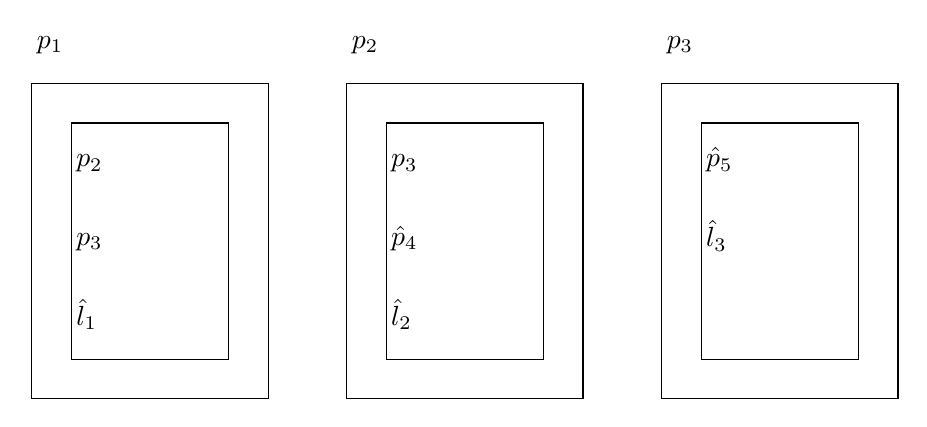
\begin{tikzpicture}
	\draw[draw=black, thin, solid] (-5.00,3.00) rectangle (-3.00,0.00);
	\draw[draw=black, thin, solid] (-1.50,3.50) rectangle (1.50,-0.50);
	\draw[draw=black, thin, solid] (2.50,3.50) rectangle (5.50,-0.50);
	\draw[draw=black, thin, solid] (-1.00,3.00) rectangle (1.00,0.00);
	\draw[draw=black, thin, solid] (3.00,3.00) rectangle (5.00,0.00);
	\draw[draw=black, thin, solid] (-5.50,3.50) rectangle (-2.50,-0.50);
	\node[black, anchor=south west] at (-5.56,3.75) {$p_1$};
	\node[black, anchor=south west] at (-1.56,3.75) {$p_2$};
	\node[black, anchor=south west] at (2.44,3.75) {$p_3$};
	\node[black, anchor=south west] at (-5.06,1.25) {$p_3$};
	\node[black, anchor=south west] at (-5.06,2.25) {$p_2$};
	\node[black, anchor=south west] at (-1.06,2.25) {$p_3$};
	\node[black, anchor=south west] at (-5.06,0.25) {$\hat l_1$};
	\node[black, anchor=south west] at (-1.06,0.25) {$\hat l_2$};
	\node[black, anchor=south west] at (2.94,1.25) {$\hat l_3$};
	\node[black, anchor=south west] at (-1.06,1.25) {$\hat p_4$};
	\node[black, anchor=south west] at (2.94,2.25) {$\hat p_5$};
\end{tikzpicture}
\caption{Przykład raportów o stanie techniki}
\label{fig:raport-ex}
\end{figure}

\subsubsection{Tworzenie grafu za pomocą danych z tabel
               raportów o stanie techniki}
\label{sec:graf-raporty}

Dane z raportów o stanie techniki tworzą graf skierowany
patentów $G$. Krawędź w takim grafie istnieje jeśli patent
$p_1$ zawiera w swoim raporcie wzmiankę o patencie~$p_2$.

Wracając do przykładu \cref{fig:raport-ex}, zastosowanie algorytmu 
tworzy graf o krawędziach $E = \{ (p_2, p_1), (p_3, p_1), (p_3, p_2) \}$ i
wierzchołkach $V = { p_1, p_2, p_3 }$.

\begin{figure}\centering
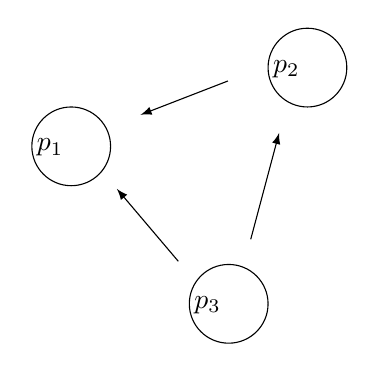
\begin{tikzpicture}
	\draw[draw=black, thin, solid] (-1.50,1.50) ellipse (0.50 and -0.50);
	\node[black, anchor=south west] at (-2.06,1.25) {$p_1$};
	\draw[draw=black, thin, solid] (1.50,2.50) ellipse (0.50 and -0.50);
	\draw[draw=black, thin, solid] (0.50,-0.50) ellipse (0.50 and -0.50);
	\node[black, anchor=south west] at (0.94,2.25) {$p_2$};
	\node[black, anchor=south west] at (-0.06,-0.75) {$p_3$};
	\draw[draw=black, -latex, thin, solid] (-0.14,0.04) -- (-0.92,0.96);
	\draw[draw=black, -latex, thin, solid] (0.78,0.32) -- (1.14,1.67);
	\draw[draw=black, -latex, thin, solid] (0.49,2.33) -- (-0.62,1.90);
\end{tikzpicture}
\caption{Graf dla przykładowego zestawu raportów \cref{fig:raport-ex}}
\label{fig:raport-ex-G}
\end{figure}

Zakładając, że wpisy ekspertów zawierają wyłącznie kody publikacji 
patentów, graf mógłby być stworzony przez bezpośrednie powiązanie
ich z danymi. Istotnym problemem w takiej sytuacji jest jakość \ac{OCR},
która jest dobra, ale nie pewna.\todonote{jakaś miara jakości}
Wpisy ekspertów nie są jednak jednorodne w taki sposób. Problem
rozpoznania znaków nie jest jedyny, bo pojawiają się kolejne:

\begin{itemize}
\item wątpliwa jakość \ac{OCR}
\item wpisy to nie tylko kody patentowe
\item wspominane kody patentowe nie zawsze są publikacjami,
      mogą to być np. kody złożenia aplikacji\todonote{przykład}
\end{itemize}

\begin{figure}[H]\centering
\includegraphics[width=0.8\textwidth]{ex-img/pat-ex-P.jpg}
\caption{Przykład odniesienia poprzez numer publikacji.}
\end{figure}

\begin{figure}[H]\centering
\includegraphics[width=0.8\textwidth]{ex-img/pat-ex-A.jpg}
\caption{Przykład odniesienia poprzez numer aplikacji.}
\end{figure}

\begin{figure}[H]\centering
\includegraphics[width=0.8\textwidth]{ex-img/pat-ex-A-P.jpg}
\caption{Przykład odniesienia poprzez numer aplikacji i publikacji
         jako jeden numer.}
\end{figure}

Sposobem na minimalizację zjawiska błędnych powiązań jest zastosowanie
algorytmu wyszukiwania (\cref{sec:wyszukiwanie}).

Ninejsze wyszukiwanie polega na wskazaniu sumy zbiorów
słów: numerów patentowych, słów języka naturalnego oraz dat. 
Wskazanie tej sumy zachodzi dla każdej pary wszystkich słów zapytań
ze wszystkimi słowami ze zbioru danych. Dodatkowo zachodzi łączenie
częściowe, które dopasowuje n-gramy poszczególnych słów. Od pewnego
minimalnego dopasowania zostają one uwzględnione. Całość wymaga
pewnych kroków optymalizacyjnych. Głównym jest zasada, że słowa
są dopasowywane tylko pod warunkiem, że zaszło dopasowanie numeru
patentu. \todonote{umieścić przykład}

W trakcie wyszukiwania tworzona jest jego punktacja, aby odróżnić
wartościowe wyniki. Oprócz punktacji jest też ustalanie poziomu
wyszukiwania na podstawie tego jakie rzeczywiste dane są łącznikami.
Wybierane są wyłącznie pojedyncze, najlepsze wyniki.\todonote{szczgł. opis}